%% REPORT_IEEE.tex  -- IEEEtran two-column conference format (trimmed to ~6 pp)
%% Build:  pdflatex REPORT_IEEE.tex  (run twice for cross-refs). Compile from repo root.
\documentclass[conference]{IEEEtran}

\usepackage{graphicx}
\usepackage{booktabs}
\usepackage{amsmath,amssymb}
\usepackage{textcomp}
\usepackage[hidelinks]{hyperref}

\graphicspath{{results/}{./}}

\begin{document}

\title{The Universality of Electricity Demand:\\
Zero-Shot Foundation Models Match Locally-Trained\\
Accuracy on Brazil's Power Grid}

\author{\IEEEauthorblockN{Nelson Barlow}
\IEEEauthorblockA{Department of [---], [University]\\
Email: qdhkbzsmzx@privaterelay.appleid.com}}

\maketitle

\begin{abstract}
Short-term load forecasting (STLF) has traditionally required models trained on years
of local historical demand---a barrier in data-scarce grids. We ask whether recent time
series \emph{foundation models}, applied zero-shot, can forecast Brazilian electricity
load with no local training. Using seven years (2019--2025) of hourly ONS load across
all four subsystems of the interconnected grid (SIN), we benchmark Chronos-2 (120\,M),
TiRex (35\,M), and Moirai 2.0 (11\,M) against a hyperparameter-tuned N-BEATS, a linear
model, an LSTM, and a seasonal-naive baseline. On the Southeast/Center-West (SE)
subsystem at a 24-hour horizon, zero-shot Chronos-2 attains 1.86\,\% MAPE---statistically
indistinguishable from a tuned N-BEATS trained on 5+ years of local data
(1.91\,\%\,$\pm$\,0.08\,\%; Diebold--Mariano $p>0.29$). Light fine-tuning yields only a
7\,\% relative gain (1.73\,\%). The result holds across all four subsystems (1.67--3.17\,\% MAPE,
$R^2>0.90$), three test years (1.89\,\%\,$\pm$\,0.04\,\%), and---on the Tokyo (TEPCO)
grid, a different country and hemisphere---where the same three zero-shot models again
beat a locally-trained N-BEATS (3.91\,\% vs.\ 4.44\,\%). The dominant residual error
concentrates on national holidays (4--5$\times$ the normal-day error); adding a single
binary holiday covariate cuts holiday error by 35\,\%. We read this as evidence for a
\emph{bounded universality} of electricity demand: physics- and behavior-driven
structure transfers across grids and hemispheres without adaptation, while
calendar-specific demand does not.
\end{abstract}

\begin{IEEEkeywords}
Short-term load forecasting, foundation models, zero-shot learning, power systems,
Chronos, Moirai, TiRex, N-BEATS.
\end{IEEEkeywords}

\section{Introduction}
Short-term load forecasting (STLF) underpins unit commitment, economic dispatch,
reserve sizing, and day-ahead market clearing. The dominant paradigm has each utility
build a bespoke model trained on years of local load, augmented with weather and
calendar features. This imposes a heavy barrier in data-scarce contexts---newly
interconnected regions, microgrids, and developing grids lacking long, clean records.

\emph{Time series foundation models} (TSFMs)---large networks pretrained on billions of
observations across diverse domains---raise a sharp question: can a model that has never
seen a particular grid's data forecast its load accurately? If so, forecasting could be
deployed without the data-collection and maintenance overhead of local training.

We frame this as a hypothesis of \emph{universality}. Demand is shaped by two kinds of
forces. The first are universal---the physics of heating, cooling, and lighting; the
circadian rhythm of activity; the weekly work/rest cycle---producing daily peaks,
overnight troughs, and weekend dips in every electrified society. The second are
local---national holidays, hydro-dependent supply constraints, and southern-hemisphere
seasonality inverted from the northern-hemisphere data these models consume. If a
pretrained model has internalized the universal component, it should transfer to an
unseen grid zero-shot, with residual error confined to the local component.

We test this primarily on the Brazilian interconnected system (SIN) using public ONS
data, with a cross-country replication on the Tokyo (TEPCO) grid. Our contributions are:
(1)~a systematic benchmark of 2024-era TSFMs on Brazilian load (all four SIN subsystems,
four horizons, three test years) plus a cross-country replication on a Japanese grid;
(2)~evidence that zero-shot models match or beat a tuned, locally-trained N-BEATS
(Diebold--Mariano $p>0.29$ on SE); (3)~a precise account of \emph{when and why} they
fail---and a holiday covariate that recovers most of the gap; and (4)~a reproducible
benchmark.

\section{Related Work}
Brazilian STLF work relies on locally-trained SVR, ANN, ARIMA, and LSTM models on ONS
or utility data \cite{santos2023,velasquez2022,oliveira2023}, all requiring per-grid
development. The TSFM paradigm emerged in 2023--2024---pretrain on billions of time
points, then forecast unseen series zero-shot---with models including Chronos
\cite{chronos}, TimesFM \cite{timesfm}, Moirai \cite{moirai}, and TiRex \cite{tirex}.
TSFMs have been evaluated on US grids (ERCOT \cite{ercot}), Singapore/Australia
\cite{exo}, and European households \cite{household}, but not on emerging-market grids
with hydro dependency, inverted seasonality, and distinct holiday calendars, nor against
a locally-trained deep-learning baseline on the same data. We fill that gap.

\section{Data and Methodology}
\textbf{Data.} Hourly load from the ONS open-data portal (dados.ons.org.br, CC-BY 4.0)
for the four SIN subsystems (Table~\ref{tab:data}); SE is the largest at $\sim$55\,\% of
national load (which averages 71{,}081\,MW). Each series spans 2019-01-01 to 2025-12-31
(61{,}368 hourly rows). The most recent 365 days (8{,}760\,h) form the test set:
foundation models see only the preceding context window (zero-shot, never trained on ONS
data); trained baselines use all earlier data, reserving the prior 60 days for
validation.

\begin{table}[t]
\centering
\caption{SIN Subsystems and Dataset Statistics (2019--2025)}
\label{tab:data}
\begin{tabular}{llrrr}
\toprule
Sub. & Region & Mean (MW) & Test (MW) & Share \\
\midrule
SE & SP, RJ, MG & 40{,}408 & 44{,}226 & $\sim$55\,\% \\
S  & PR, SC, RS & 12{,}320 & 13{,}804 & $\sim$17\,\% \\
NE & BA, PE, CE & 11{,}711 & 13{,}267 & $\sim$17\,\% \\
N  & AM, PA     &  6{,}641 &  8{,}312 & $\sim$11\,\% \\
\bottomrule
\end{tabular}
\end{table}

\textbf{Task.} Given a context window of hourly load, predict the next 24\,h
(day-ahead); we also evaluate 168/336/720\,h. Forecasts roll through the test year in
24-h steps and are averaged.

\textbf{Models.} Zero-shot: \emph{Chronos-2} (120\,M, encoder-only, quantile output;
median reported), \emph{TiRex} (35\,M, xLSTM), \emph{Moirai 2.0} (11\,M). We verified
ONS data is \emph{absent} from Chronos's pretraining corpus \cite{chronos,bolt}
(no data leakage). Trained: \emph{N-BEATS} (7.3\,M, Darts; primary baseline),
\emph{Linear} ($\sim$8\,K), \emph{LSTM}, and \emph{Naive (7-day-ago)}. Metrics: MAE,
RMSE (MW), MAPE, MASE/RMSSE (seasonality\,=\,24), $R^2$; CRPS and prediction intervals
for probabilistic eval; Diebold--Mariano (DM) test on per-window errors. Hardware:
Mac~Mini~M4, no GPU; MPS fails for Darts N-BEATS and Chronos fine-tuning, run on CPU.

\section{Results}
\subsection{Main Comparison (SE, 24\,h)}
Table~\ref{tab:main} and Fig.~\ref{fig:se24} report the headline. Zero-shot Chronos-2
achieves \textbf{1.86\,\% MAPE}, edging out a tuned N-BEATS (1.91\,\%) trained on five
years of local data, with Moirai close behind (1.93\,\%); all TSFMs beat naive
(5.13\,\%) by a wide margin. The DM test gives $p>0.29$ against all three N-BEATS seeds
and bootstrap 95\,\% CIs overlap (Chronos-2 CI $[1.70\%,2.04\%]$): Chronos-2 vs.\
N-BEATS is a \emph{statistical tie}---but Chronos-2 needs \emph{zero} local training.
Light fine-tuning (400 steps, lr 1e-5, $\sim$40\,min CPU) reaches 1.73\,\% (a 7\,\%
gain), showing pretraining already captures the dominant patterns. The LSTM failed to
train competitively and is shown for completeness. For context, Chronos-2 (load only)
rivals proprietary ISO systems using weather/calendar inputs: PJM 24\,h
(1.78--1.98\,\%), ERCOT (1.66--3.73\,\%).

\begin{table}[t]
\centering
\caption{Main Results --- SE, 24\,h Horizon}
\label{tab:main}
\begin{tabular}{llrrr}
\toprule
Model & Type & MAPE\,\% & MASE & $R^2$ \\
\midrule
\textbf{Chronos-2} & \textbf{Fine-tuned} & \textbf{1.73} & 0.30 & 0.96 \\
Chronos-2 & Zero-shot & 1.86 & 0.33 & 0.96 \\
N-BEATS (tuned) & Trained 5\,yr & 1.91\,$\pm$\,0.08 & 0.34 & 0.96 \\
Moirai 2.0 & Zero-shot & 1.93 & 0.34 & 0.95 \\
Linear & Trained & 2.26 & 0.40 & 0.94 \\
TiRex & Zero-shot & 2.33 & 0.40 & 0.94 \\
Naive (7\,d) & Baseline & 5.13 & 0.89 & 0.77 \\
LSTM & Trained & 13.14 & 2.39 & $-0.36$ \\
\bottomrule
\end{tabular}
\end{table}

\begin{figure}[t]
\centering
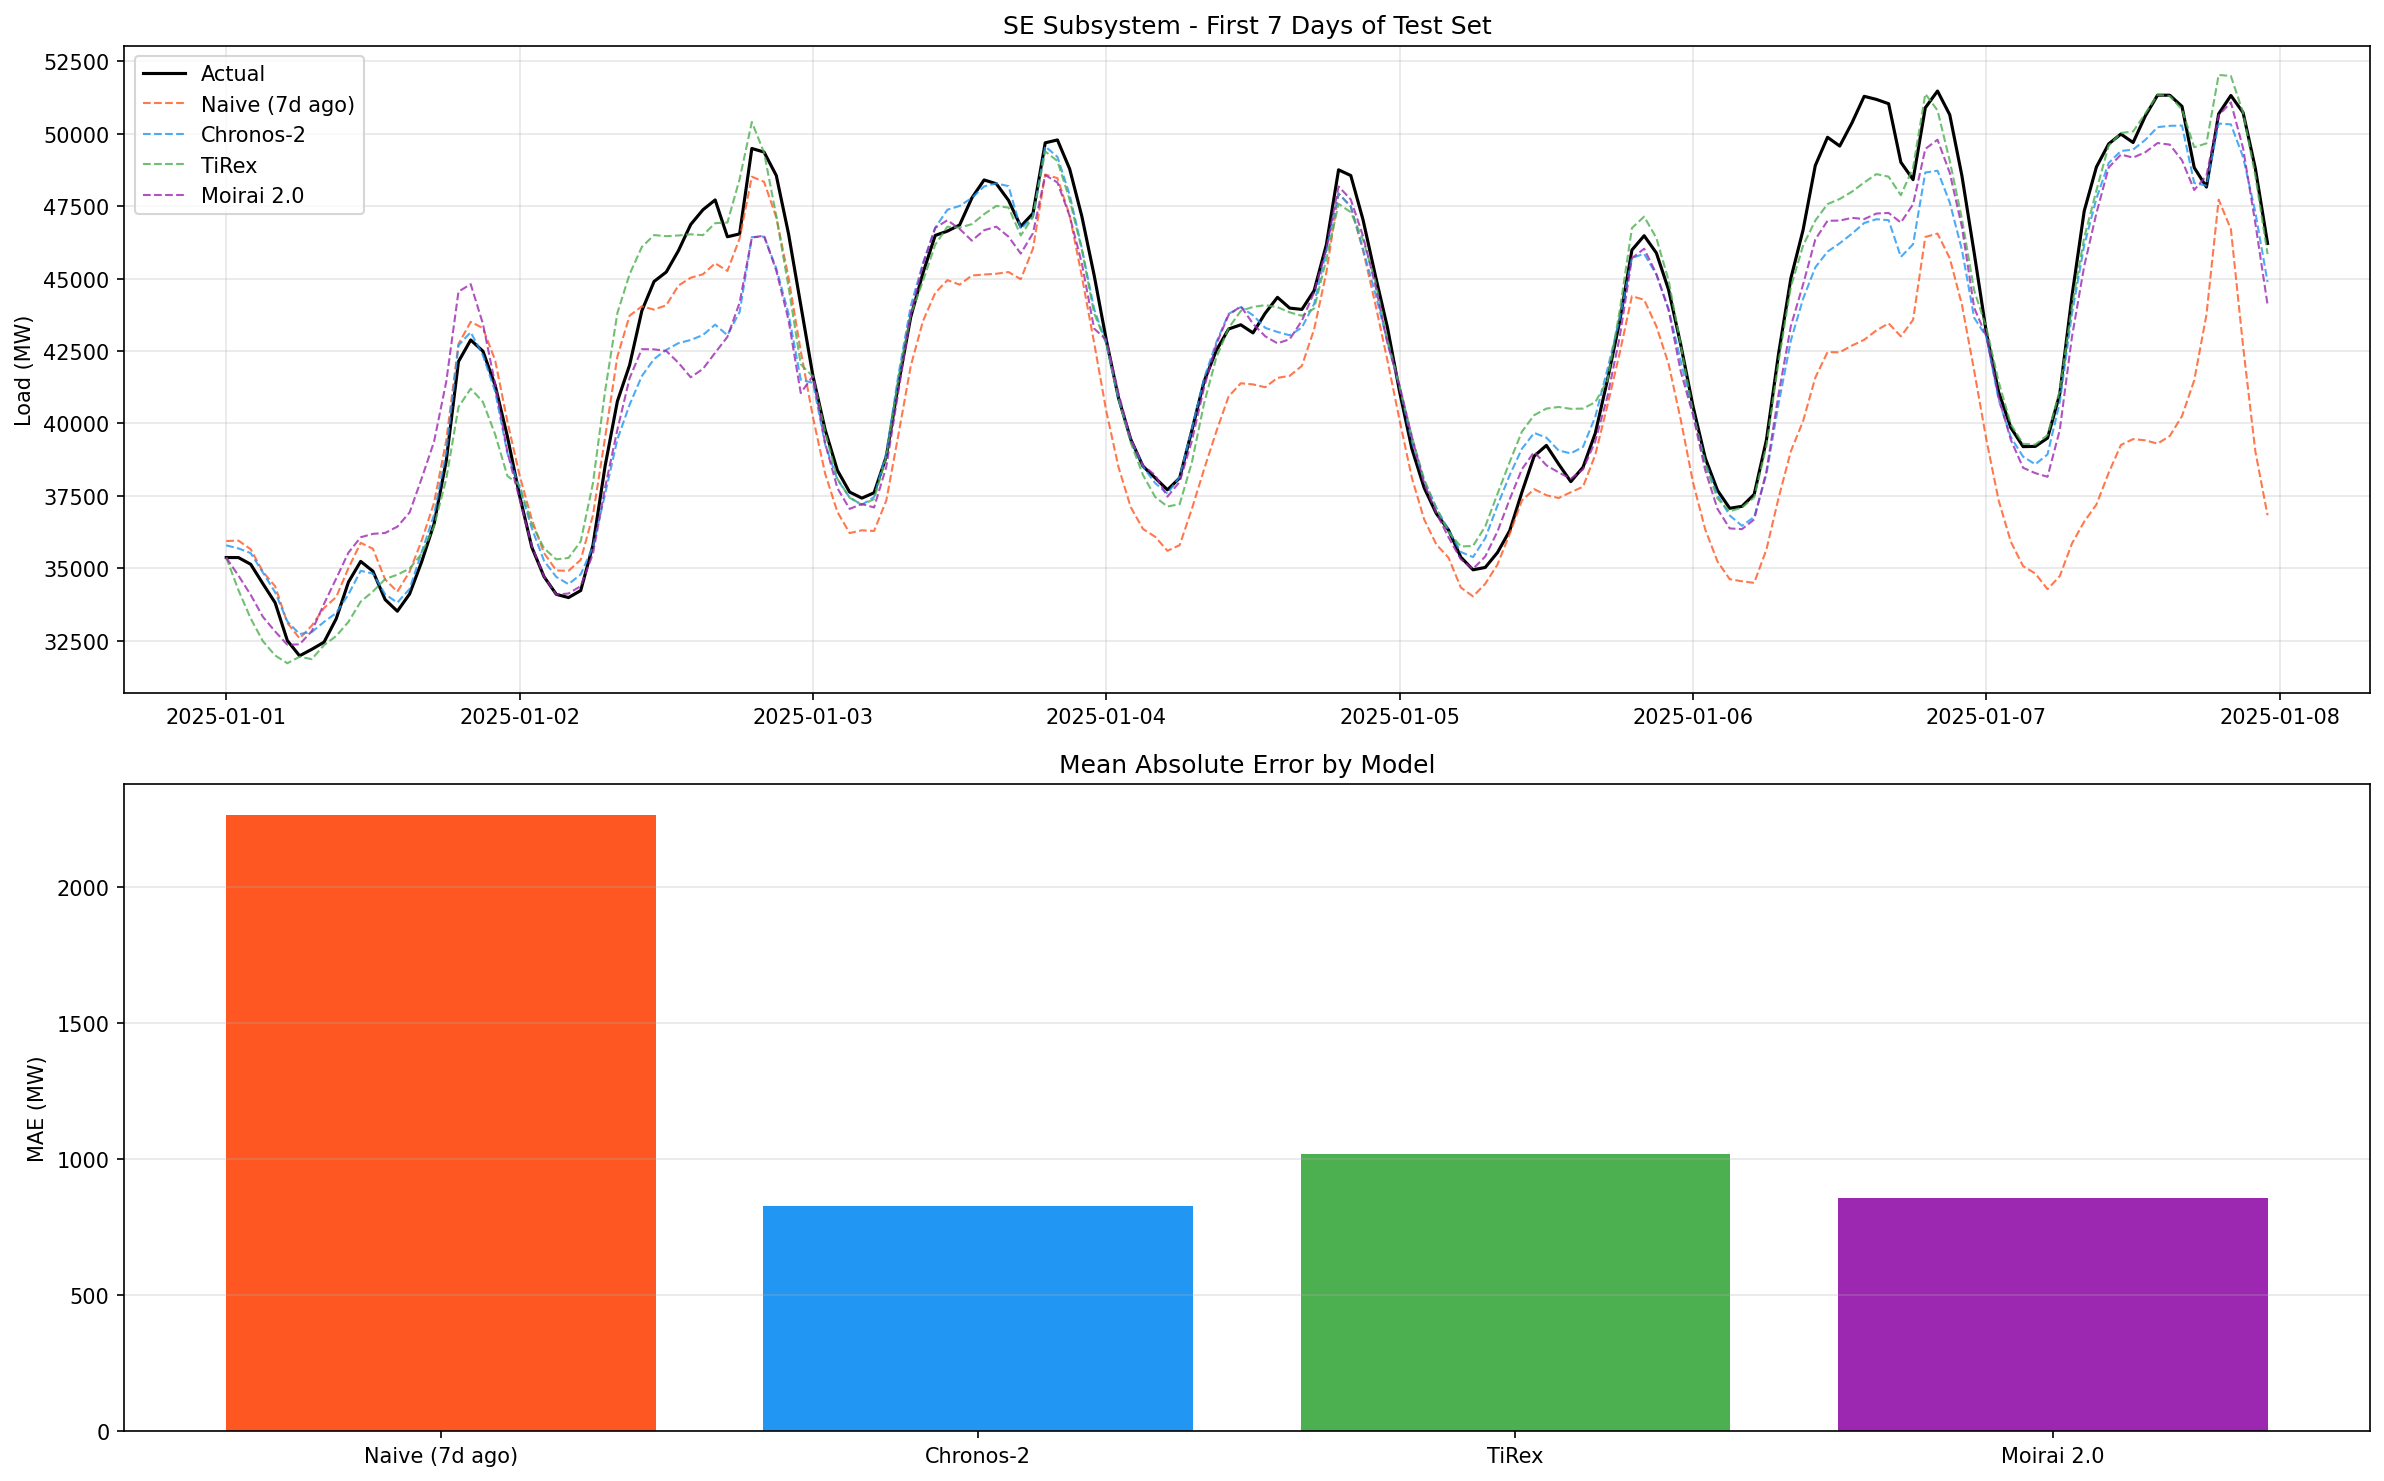
\includegraphics[width=\columnwidth]{benchmark_SE_24h.png}
\caption{SE, 24\,h: 7-day forecast comparison and per-model MAE. Zero-shot Chronos-2
tracks the load curve closely; the naive baseline lags on the daily ramp.}
\label{fig:se24}
\end{figure}

\emph{N-BEATS tuning.} To ensure fairness, N-BEATS was grid-searched over input length
$\in\{168,336,720\}$\,h and lr $\in\{$1e-4, 5e-4, 1e-3$\}$. The best config (168\,h,
lr 5e-4), re-run with seeds $\{42,123,7\}$, gives 1.85/1.88/2.00\,\%
$\rightarrow$ \textbf{1.91\,\%\,$\pm$\,0.08\,\%}---a 0.23\,pp improvement over its
untuned setting (2.14\,\%), confirming the baseline is properly optimized.

\subsection{Generalization}
\textbf{Across subsystems.} Chronos-2 leads on all four (Table~\ref{tab:subs}),
45--64\,\% above naive, $R^2>0.90$ everywhere. The smallest subsystem (N) is easiest
(1.67\,\%); S is hardest (3.17\,\%), likely from winter cold-front heating. On S, tuned
N-BEATS reaches 3.26\,\%\,$\pm$\,0.21\,\% vs.\ 3.17\,\%---again a tie.

\begin{table}[t]
\centering
\caption{MAPE (\%) by Subsystem --- 24\,h}
\label{tab:subs}
\begin{tabular}{lrrrr}
\toprule
Sub. & Naive & Chronos-2 & TiRex & Moirai \\
\midrule
SE & 5.13 & \textbf{1.86} & 2.33 & 1.93 \\
S  & 7.11 & \textbf{3.17} & 3.37 & 3.35 \\
NE & 3.76 & \textbf{1.94} & 2.06 & 2.05 \\
N  & 3.03 & \textbf{1.67} & 1.67 & 1.76 \\
\bottomrule
\end{tabular}
\end{table}

\textbf{Horizon.} Accuracy degrades with horizon, with a \emph{naive crossover} at
$\sim$2--3 weeks. SE Chronos-2 MAPE: 1.86\,\% (24\,h), 3.59\,\% (168\,h), 4.18\,\%
(336\,h), 5.69\,\% (720\,h); at 720\,h Chronos-2 (MASE 1.02) and Moirai (1.03) fall
behind naive while only TiRex (0.91) stays ahead. TSFMs are thus best for operational
(24--168\,h) horizons.

\textbf{Multi-year.} Chronos-2 is stable across test years 2023/2024/2025
(1.94/1.87/1.86\,\%, mean 1.89\,\%\,$\pm$\,0.04\,\%) while naive varies more
(5.31\,\%\,$\pm$\,0.17\,\%).

\textbf{Context length.} The critical threshold is \emph{one week}: MAPE halves
(5.65\,\%$\rightarrow$2.80\,\%) once a full weekly cycle is seen, reaching 1.86\,\% at
30 days; beyond that, returns are marginal (90 days: 1.77\,\%). Thirty days is the
practical accuracy/compute sweet spot.

\textbf{Model scale.} The Chronos-Bolt family scales log-linearly
(Fig.~\ref{fig:scaling}): Tiny~9\,M~$\to$~2.28\,\%, Mini~21\,M~$\to$~2.19\,\%,
Small~48\,M~$\to$~2.02\,\%, Chronos-2~120\,M~$\to$~1.86\,\%. At matched size zero-shot
Bolt-Tiny (2.28\,\%) loses to tuned N-BEATS (1.91\,\%), but Moirai (11\,M, 1.93\,\%)
nearly ties it---architecture matters as much as scale.

\begin{figure}[t]
\centering
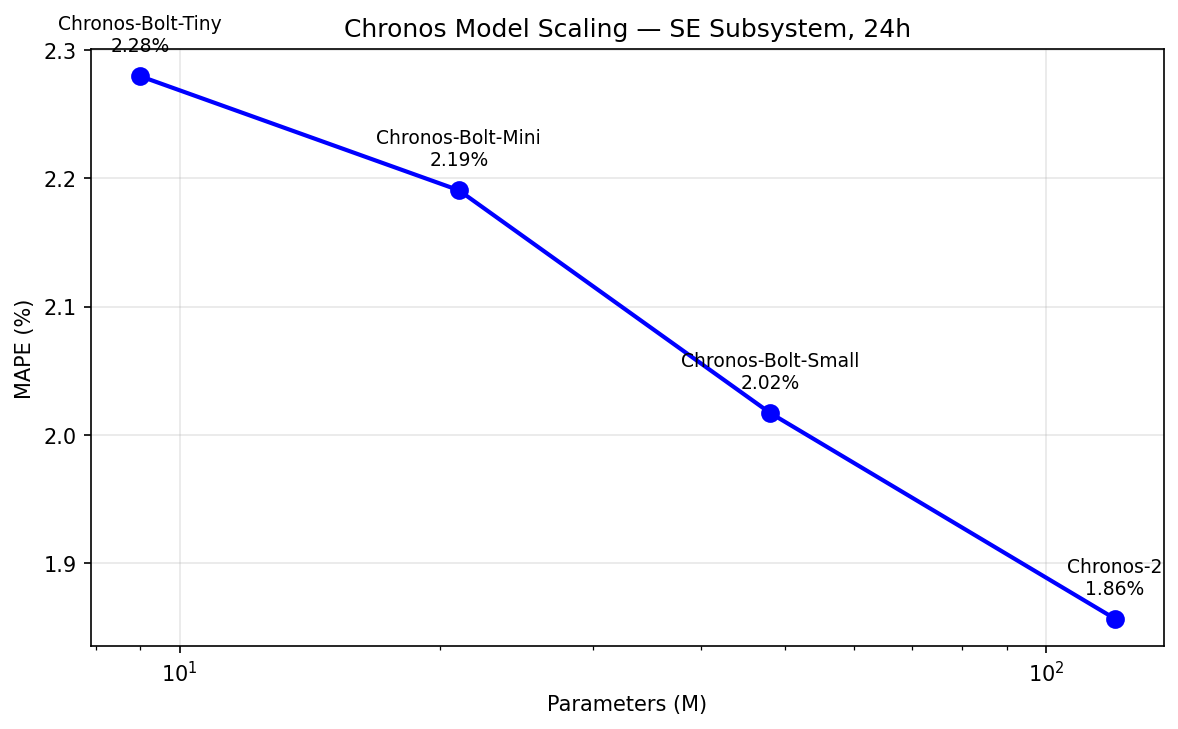
\includegraphics[width=\columnwidth]{chronos_scaling_SE_24h.png}
\caption{Chronos scaling: MAPE decreases log-linearly with parameter count; at
$\sim$9\,M zero-shot trails tuned N-BEATS, and by 120\,M it closes the gap.}
\label{fig:scaling}
\end{figure}

\textbf{Probabilistic.} Both probabilistic models are well-calibrated but slightly
conservative---80\,\% PIs cover 86--89\,\% of outcomes, desirable for reserve
scheduling. Chronos-2 has the better CRPS (643 vs.\ 688\,MW) and Winkler score (4354
vs.\ 4378); Moirai produces sharper intervals (3024 vs.\ 3295\,MW) despite being
11$\times$ smaller.

\subsection{Cross-Country Replication (Tokyo)}
To probe universality beyond Brazil, we repeat the benchmark on the TEPCO grid (Tokyo,
$\sim$32\,GW, 2019--2024), with N-BEATS trained on 2019--2023 Japanese data and 2024 held
out (Table~\ref{tab:tepco}). All three zero-shot foundation models again \emph{beat} the
locally-trained N-BEATS, in the identical ranking observed for Brazil (Chronos-2 $>$
Moirai $>$ TiRex $\gg$ naive). Absolute MAPE is higher (Japanese demand is more volatile),
but the qualitative result---zero-shot transfer matches or exceeds dedicated local
training---holds across a different country, hemisphere, and holiday calendar. This is the
strongest single piece of evidence for the universality hypothesis.

\begin{table}[t]
\centering
\caption{Cross-Country: TEPCO Tokyo --- 24\,h, test 2024}
\label{tab:tepco}
\begin{tabular}{llrrr}
\toprule
Model & Type & MAPE\,\% & MASE & $R^2$ \\
\midrule
Chronos-2  & Zero-shot      & \textbf{3.91} & 0.59 & 0.91 \\
Moirai 2.0 & Zero-shot      & 3.94 & 0.59 & 0.91 \\
TiRex      & Zero-shot      & 4.05 & 0.61 & 0.91 \\
N-BEATS    & Trained 5\,yr  & 4.44 & 0.67 & 0.89 \\
Naive (7\,d) & Baseline     & 8.86 & 1.30 & 0.65 \\
\bottomrule
\end{tabular}
\end{table}

\section{Error Analysis: When and Why}
Error follows the load curve (Fig.~\ref{fig:error}): lowest in the overnight trough
(0.51\,\% at hour 0), highest mid-afternoon (2.72\,\% at hour 15). Weekends (1.75\,\%)
beat weekdays (1.90\,\%); Monday is hardest (2.37\,\%), Tuesday easiest (1.60\,\%).

The central finding is the holiday regime (Table~\ref{tab:holiday}). On Brazilian public
holidays Chronos-2 degrades to several times its normal-day error, because nothing in the
global corpus signals a Brazilian holiday, so it forecasts ordinary workday demand. The
effect is a property of the data, not one model: on the same holidays Moirai reaches
7.9\,\% and TiRex 9.1\,\% MAPE, and the naive baseline 12.8\,\%, against $\sim$1.6\,\% on
normal days.

This is precisely where a small dose of local knowledge should help---and it does. Adding
a single binary holiday covariate and lightly fine-tuning Chronos-2 (test 2024) cuts
holiday MAPE by 35\,\% (6.76\,\%\,$\rightarrow$\,4.37\,\%), Carnaval by 18\,\%, and the
day after a holiday by 16\,\%, while normal days are untouched and overall MAPE falls
5\,\% (Table~\ref{tab:holiday}). The lone regression---``bridge'' days between a holiday
and a weekend worsen (3.02\,\%\,$\rightarrow$\,6.12\,\%), on only 24 test hours---marks
where the coarse binary encoding is too blunt and a richer calendar feature is needed.
This is exactly the bounded-universality prediction: the residual error is local calendar
knowledge, and supplying that knowledge recovers most of the gap.

\begin{table}[t]
\centering
\caption{Holiday Covariate Experiment --- Chronos-2, SE (test 2024)}
\label{tab:holiday}
\begin{tabular}{lrrrr}
\toprule
Regime & Hours & Zero-shot & +\,Cov. & $\Delta$\,\% \\
\midrule
Normal      & 5688 & 1.53 & 1.53 & $+0.0$ \\
Weekend     & 2232 & 1.77 & 1.74 & $-2.0$ \\
Day-before  &  264 & 2.28 & 2.19 & $-4.2$ \\
Day-after   &  264 & 2.29 & 1.93 & $-15.8$ \\
Carnaval    &   48 & 5.68 & 4.64 & $-18.3$ \\
\textbf{Holiday} & 264 & \textbf{6.76} & \textbf{4.37} & $\mathbf{-35.4}$ \\
Bridge      &   24 & 3.02 & 6.12 & $+102.5$ \\
\midrule
Overall     & 8784 & 1.82 & 1.73 & $-5.0$ \\
\bottomrule
\end{tabular}
\end{table}

\begin{figure}[t]
\centering
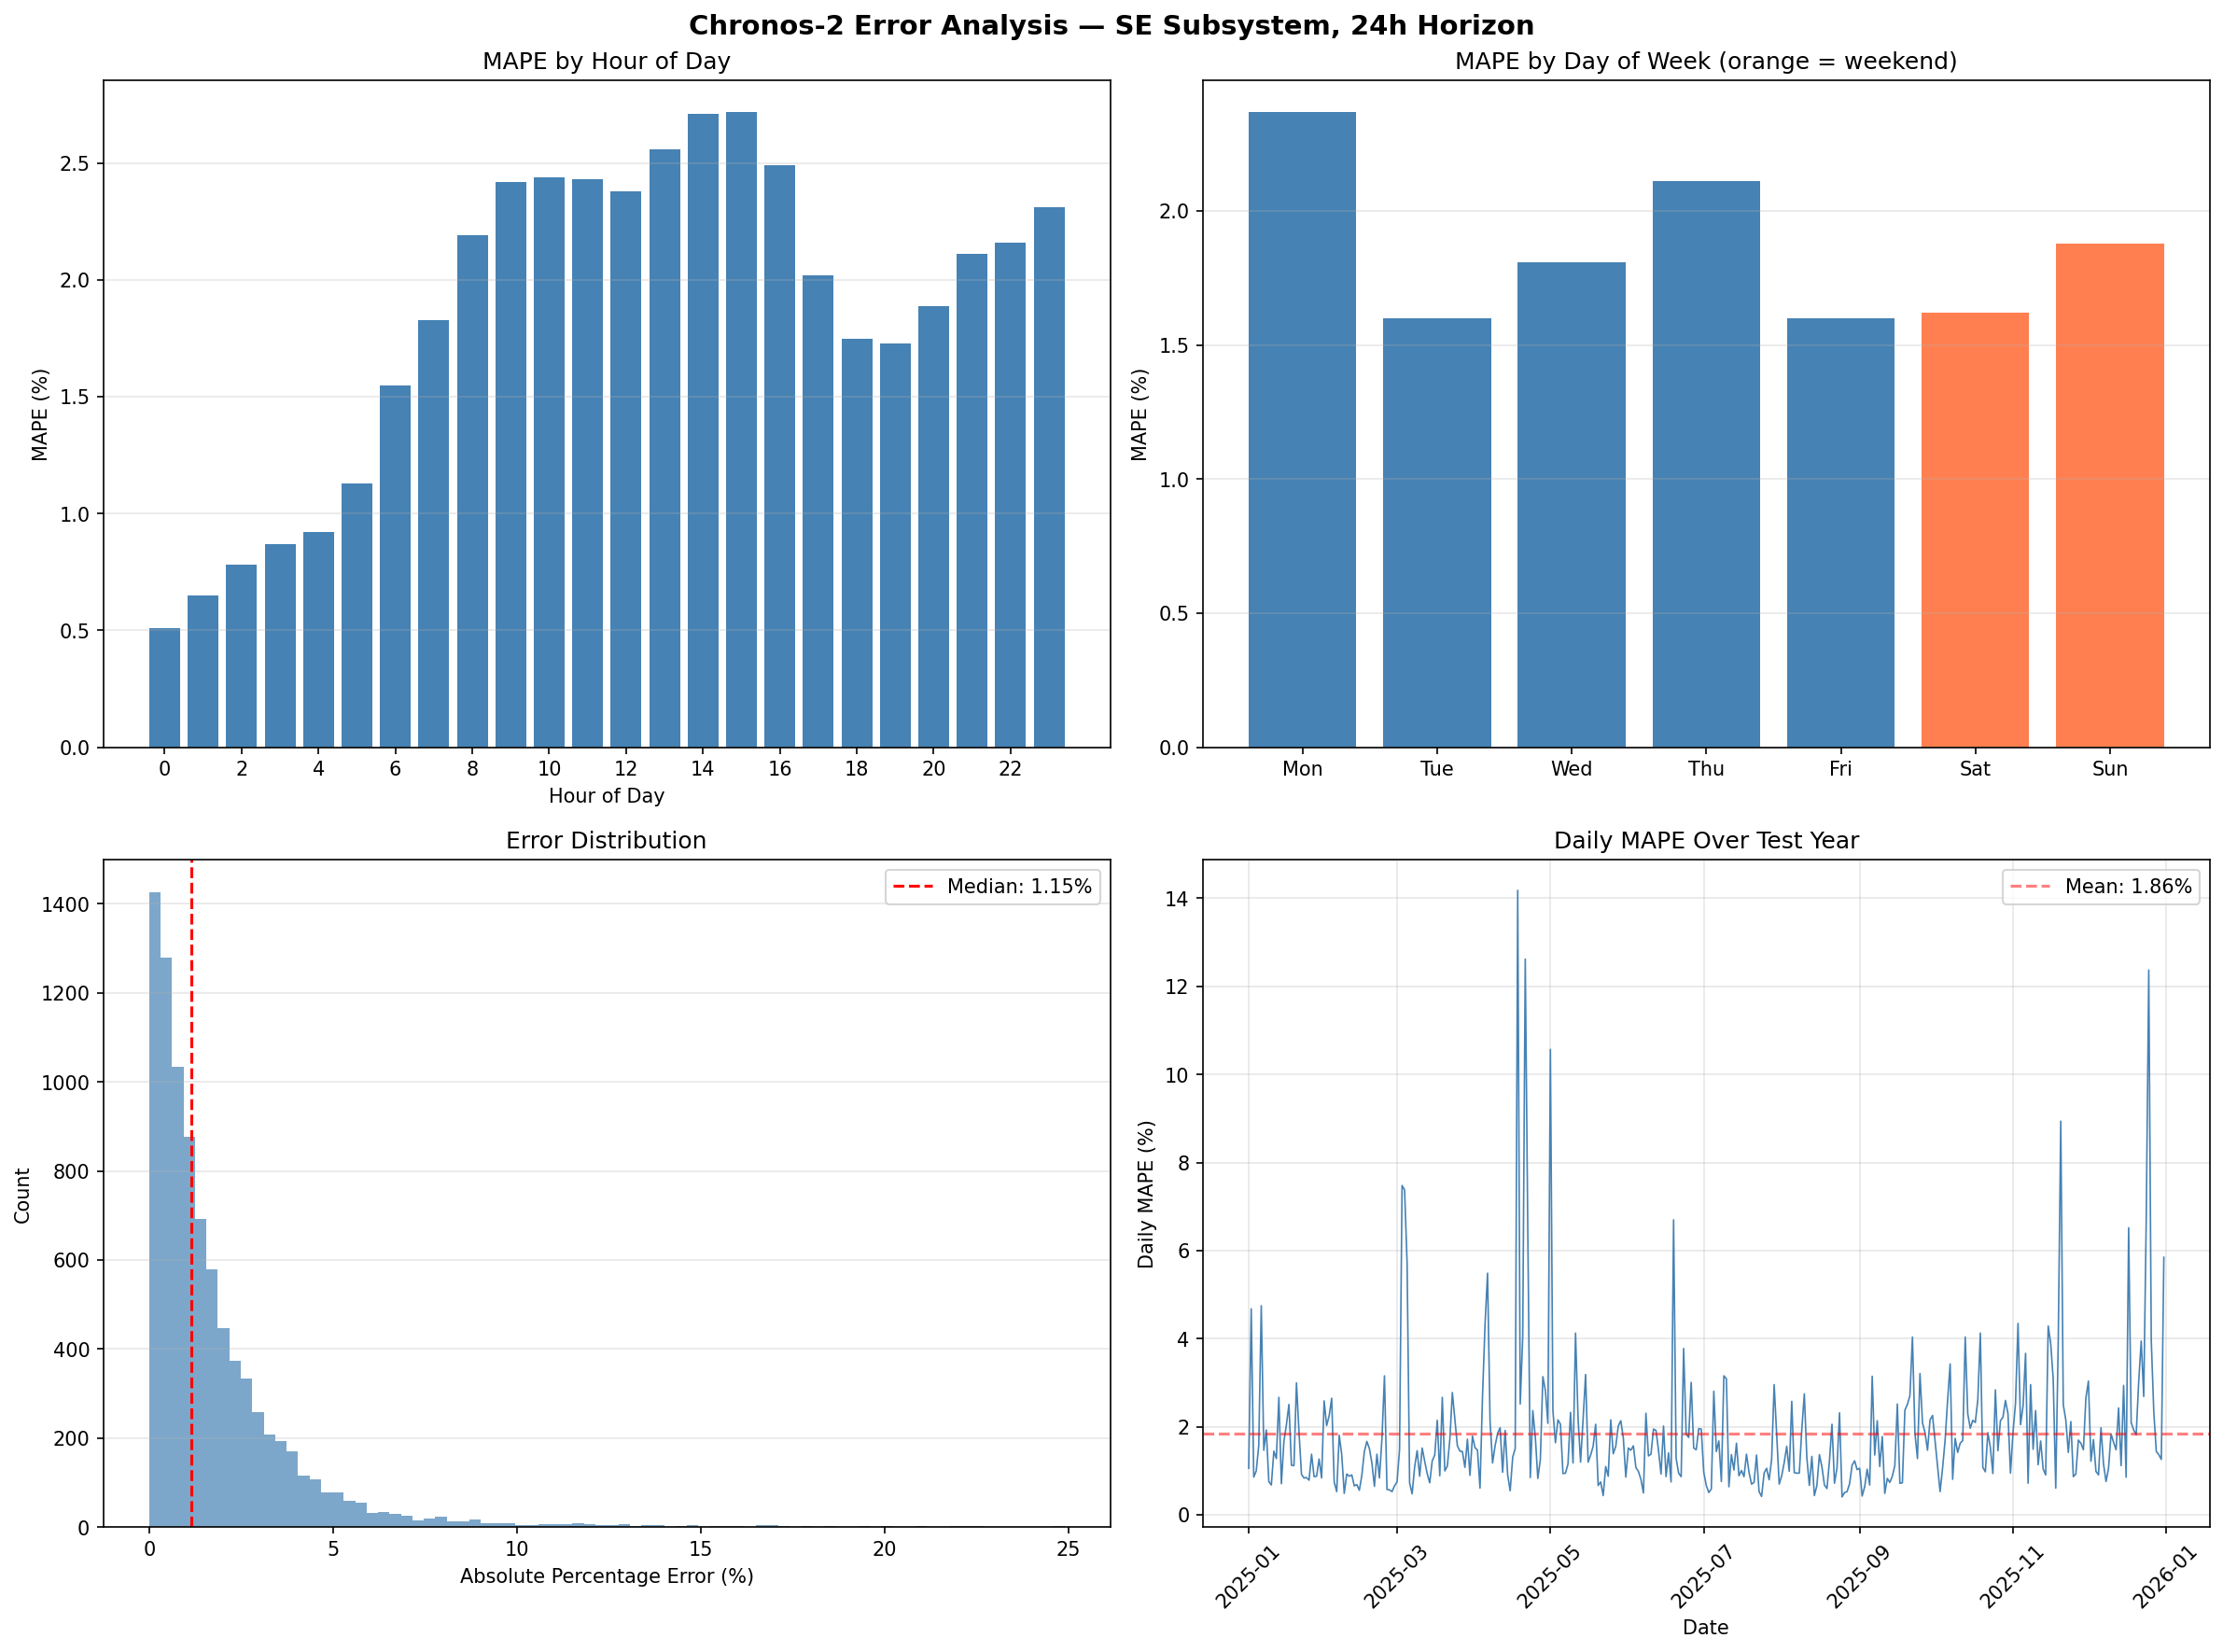
\includegraphics[width=\columnwidth]{error_analysis_SE.png}
\caption{Error decomposition: MAPE by hour-of-day and day-of-week, error distribution,
and daily MAPE over the test year (spikes coincide with holidays).}
\label{fig:error}
\end{figure}

\section{Discussion and Conclusion}
The results support a universality of electricity demand \emph{with a precise boundary}.
Components driven by shared physical and behavioral forces---diurnal cycles, the
workweek, seasonality---transfer to an unseen grid well enough that a zero-shot model
ties or beats a locally-trained one across subsystems, years, and---on the Tokyo
grid---a second country and hemisphere. Components driven by local culture---national
holidays---do not, degrading 4--5$\times$; but supplying exactly that local knowledge via
a binary holiday covariate recovers 35\,\% of the holiday gap, confirming the boundary is
calendar knowledge rather than an architectural limit.

This yields an operational recipe: (1)~start zero-shot (Chronos-2, or the 11\,M Moirai
when resource-constrained) with $\sim$30 days of context; (2)~fine-tune if resources
permit ($\sim$7\,\% gain, 40\,min CPU); (3)~add a binary holiday covariate (cut holiday
error 35\,\% in our experiment); (4)~do not use beyond $\sim$2 weeks, where naive wins;
(5)~one week of history is the minimum viable context. \emph{Limitations:} univariate
input (no weather); two countries (Brazil, Japan) remain a small sample of grids;
load-only trained baselines, so a weather-augmented TFT could narrow the gap; the
holiday covariate's binary encoding regresses on rare ``bridge'' days; and the LSTM did
not converge competitively.

In sum, a model pretrained on global time series, with no exposure to the target grid's
data, matches a tuned model trained on 5+ years of local Brazilian data
(1.86\,\% vs.\ 1.91\,\%\,$\pm$\,0.08\,\%; DM $p>0.29$) across all four subsystems and
three years, and \emph{beats} a locally-trained N-BEATS on the Tokyo grid (3.91\,\% vs.\
4.44\,\%). The boundary of universality is precise---the model fails on culturally-local
holidays and essentially nowhere else---and a single holiday covariate largely closes
even that gap. For operators in data-scarce grids, accurate day-ahead forecasting no
longer requires years of local model development: thirty days of load history and an
off-the-shelf foundation model suffice.

\section*{Acknowledgment}
The author thanks the course instructor for suggesting cross-market generalization (an
Asian-market extension is in progress) and reviewers for the N-BEATS tuning and
data-leakage audits incorporated above.

\begin{thebibliography}{99}
\bibitem{chronos} A.~F. Ansari \emph{et al.}, ``Chronos: Learning the language of time series,'' \emph{TMLR}, 2024 (arXiv:2403.07815).
\bibitem{bolt} A.~F. Ansari \emph{et al.}, ``Chronos-Bolt: Efficient and scalable time series forecasting,'' 2025 (arXiv:2510.15821).
\bibitem{timesfm} A.~Das \emph{et al.}, ``A decoder-only foundation model for time-series forecasting,'' \emph{ICML}, 2024.
\bibitem{moirai} G.~Woo \emph{et al.}, ``Moirai: A time series foundation model for universal forecasting,'' \emph{ICML}, 2024.
\bibitem{tirex} NX-AI, ``TiRex: xLSTM-based time series foundation model,'' \emph{NeurIPS}, 2025.
\bibitem{santos2023} L.~C.~B. Santos \emph{et al.}, ``An overview of short-term load forecasting for electricity systems operational planning,'' \emph{Energies}, vol.~16, no.~21, 7444, 2023.
\bibitem{velasquez2022} C.~E. Velasquez \emph{et al.}, ``Analysis of time series models for Brazilian electricity demand forecasting,'' \emph{Energy}, vol.~247, 123483, 2022.
\bibitem{oliveira2023} E.~M. de Oliveira \emph{et al.}, ``Short-term load forecasting using neural networks and global climate models,'' \emph{Applied Energy}, vol.~348, 121439, 2023.
\bibitem{ercot} Q.~Xu \emph{et al.}, ``Foundation models for electricity load forecasting on ERCOT,'' 2025 (arXiv:2602.10848).
\bibitem{exo} Y.~Zhang \emph{et al.}, ``Electricity demand forecasting with exogenous data in TSFMs,'' 2025 (arXiv:2602.05390).
\bibitem{household} Z.~Zhou \emph{et al.}, ``Benchmarking TSFMs for household electricity load forecasting,'' 2024 (arXiv:2410.09487).
\end{thebibliography}

\end{document}
